\documentclass[twoside]{book}

% Packages required by doxygen
\usepackage{calc}
\usepackage{doxygen}
\usepackage{graphicx}
\usepackage[utf8]{inputenc}
\usepackage{makeidx}
\usepackage{multicol}
\usepackage{multirow}
\usepackage{fixltx2e}
\PassOptionsToPackage{warn}{textcomp}
\usepackage{textcomp}
\usepackage[nointegrals]{wasysym}
\usepackage[table]{xcolor}

% Font selection
\usepackage[T1]{fontenc}
\usepackage{mathptmx}
\usepackage[scaled=.90]{helvet}
\usepackage{courier}
\usepackage{amssymb}
\usepackage{sectsty}
\renewcommand{\familydefault}{\sfdefault}
\allsectionsfont{%
  \fontseries{bc}\selectfont%
  \color{darkgray}%
}
\renewcommand{\DoxyLabelFont}{%
  \fontseries{bc}\selectfont%
  \color{darkgray}%
}
\newcommand{\+}{\discretionary{\mbox{\scriptsize$\hookleftarrow$}}{}{}}

% Page & text layout
\usepackage{geometry}
\geometry{%
  a4paper,%
  top=2.5cm,%
  bottom=2.5cm,%
  left=2.5cm,%
  right=2.5cm%
}
\tolerance=750
\hfuzz=15pt
\hbadness=750
\setlength{\emergencystretch}{15pt}
\setlength{\parindent}{0cm}
\setlength{\parskip}{0.2cm}
\makeatletter
\renewcommand{\paragraph}{%
  \@startsection{paragraph}{4}{0ex}{-1.0ex}{1.0ex}{%
    \normalfont\normalsize\bfseries\SS@parafont%
  }%
}
\renewcommand{\subparagraph}{%
  \@startsection{subparagraph}{5}{0ex}{-1.0ex}{1.0ex}{%
    \normalfont\normalsize\bfseries\SS@subparafont%
  }%
}
\makeatother

% Headers & footers
\usepackage{fancyhdr}
\pagestyle{fancyplain}
\fancyhead[LE]{\fancyplain{}{\bfseries\thepage}}
\fancyhead[CE]{\fancyplain{}{}}
\fancyhead[RE]{\fancyplain{}{\bfseries\leftmark}}
\fancyhead[LO]{\fancyplain{}{\bfseries\rightmark}}
\fancyhead[CO]{\fancyplain{}{}}
\fancyhead[RO]{\fancyplain{}{\bfseries\thepage}}
\fancyfoot[LE]{\fancyplain{}{}}
\fancyfoot[CE]{\fancyplain{}{}}
\fancyfoot[RE]{\fancyplain{}{\bfseries\scriptsize Generated on Fri Oct 31 2014 18\+:28\+:40 for My Project by Doxygen }}
\fancyfoot[LO]{\fancyplain{}{\bfseries\scriptsize Generated on Fri Oct 31 2014 18\+:28\+:40 for My Project by Doxygen }}
\fancyfoot[CO]{\fancyplain{}{}}
\fancyfoot[RO]{\fancyplain{}{}}
\renewcommand{\footrulewidth}{0.4pt}
\renewcommand{\chaptermark}[1]{%
  \markboth{#1}{}%
}
\renewcommand{\sectionmark}[1]{%
  \markright{\thesection\ #1}%
}

% Indices & bibliography
\usepackage{natbib}
\usepackage[titles]{tocloft}
\setcounter{tocdepth}{3}
\setcounter{secnumdepth}{5}
\makeindex

% Hyperlinks (required, but should be loaded last)
\usepackage{ifpdf}
\ifpdf
  \usepackage[pdftex,pagebackref=true]{hyperref}
\else
  \usepackage[ps2pdf,pagebackref=true]{hyperref}
\fi
\hypersetup{%
  colorlinks=true,%
  linkcolor=blue,%
  citecolor=blue,%
  unicode%
}

% Custom commands
\newcommand{\clearemptydoublepage}{%
  \newpage{\pagestyle{empty}\cleardoublepage}%
}


%===== C O N T E N T S =====

\begin{document}

% Titlepage & ToC
\hypersetup{pageanchor=false,
             bookmarks=true,
             bookmarksnumbered=true,
             pdfencoding=unicode
            }
\pagenumbering{roman}
\begin{titlepage}
\vspace*{7cm}
\begin{center}%
{\Large My Project }\\
\vspace*{1cm}
{\large Generated by Doxygen 1.8.7}\\
\vspace*{0.5cm}
{\small Fri Oct 31 2014 18:28:40}\\
\end{center}
\end{titlepage}
\clearemptydoublepage
\tableofcontents
\clearemptydoublepage
\pagenumbering{arabic}
\hypersetup{pageanchor=true}

%--- Begin generated contents ---
\chapter{Todo List}
\label{todo}
\hypertarget{todo}{}

\begin{DoxyRefList}
\item[\label{todo__todo000001}%
\hypertarget{todo__todo000001}{}%
Class \hyperlink{class_j_g_meta_steam}{J\+G\+Meta\+Steam} ]sort the globbing 

sort the web calling and parsing 

sort json import and e3xport 

sort the random game execution  
\item[\label{todo__todo000006}%
\hypertarget{todo__todo000006}{}%
Member \hyperlink{class_j_g_meta_steam_1_1_j_g_meta_steam_a6785278af924d86ce5fd915d0d521f14}{J\+G\+Meta\+Steam.J\+G\+Meta\+Steam.all\+Games} ]implement  
\item[\label{todo__todo000004}%
\hypertarget{todo__todo000004}{}%
Member \hyperlink{class_j_g_meta_steam_1_1_j_g_meta_steam_a8d61d2e7e511e8001ad0de115266ce5b}{J\+G\+Meta\+Steam.J\+G\+Meta\+Steam.find\+\_\+installed\+\_\+games} ]implement  
\item[\label{todo__todo000002}%
\hypertarget{todo__todo000002}{}%
Member \hyperlink{class_j_g_meta_steam_1_1_j_g_meta_steam_ad61c5083ca71695f1d5945707c0857ae}{J\+G\+Meta\+Steam.J\+G\+Meta\+Steam.find\+\_\+steam} ]implement  
\item[\label{todo__todo000003}%
\hypertarget{todo__todo000003}{}%
Member \hyperlink{class_j_g_meta_steam_1_1_j_g_meta_steam_a589b698d11b79971bde98e61c3ab25c3}{J\+G\+Meta\+Steam.J\+G\+Meta\+Steam.find\+\_\+steam\+\_\+folders} ]implement  
\item[\label{todo__todo000005}%
\hypertarget{todo__todo000005}{}%
Member \hyperlink{class_j_g_meta_steam_1_1_j_g_meta_steam_abcb0c088945b4058f711e62e91679664}{J\+G\+Meta\+Steam.J\+G\+Meta\+Steam.game\+\_\+info} ]implement  
\item[\label{todo__todo000007}%
\hypertarget{todo__todo000007}{}%
Member \hyperlink{class_j_g_meta_steam_1_1_j_g_meta_steam_a6a34f50ae4397170316bee6f81cabbe9}{J\+G\+Meta\+Steam.J\+G\+Meta\+Steam.scrape\+\_\+info} ]implement 
\end{DoxyRefList}
\chapter{Namespace Index}
\section{Namespace List}
Here is a list of all namespaces with brief descriptions\+:\begin{DoxyCompactList}
\item\contentsline{section}{\hyperlink{namespaceall_game_parse}{all\+Game\+Parse} }{\pageref{namespaceall_game_parse}}{}
\item\contentsline{section}{\hyperlink{namespace_j_g_meta_steam}{J\+G\+Meta\+Steam} }{\pageref{namespace_j_g_meta_steam}}{}
\item\contentsline{section}{\hyperlink{namespacemeta_steam}{meta\+Steam} }{\pageref{namespacemeta_steam}}{}
\item\contentsline{section}{\hyperlink{namespacetest_request}{test\+Request} }{\pageref{namespacetest_request}}{}
\end{DoxyCompactList}

\chapter{Class Index}
\section{Class List}
Here are the classes, structs, unions and interfaces with brief descriptions\+:\begin{DoxyCompactList}
\item\contentsline{section}{\hyperlink{class_j_g_meta_steam_1_1_j_g_meta_steam}{J\+G\+Meta\+Steam.\+J\+G\+Meta\+Steam} }{\pageref{class_j_g_meta_steam_1_1_j_g_meta_steam}}{}
\item\contentsline{section}{\hyperlink{class_j_g_meta_steam}{J\+G\+Meta\+Steam} }{\pageref{class_j_g_meta_steam}}{}
\end{DoxyCompactList}

\chapter{File Index}
\section{File List}
Here is a list of all files with brief descriptions\+:\begin{DoxyCompactList}
\item\contentsline{section}{\hyperlink{all_game_parse_8py}{all\+Game\+Parse.\+py} }{\pageref{all_game_parse_8py}}{}
\item\contentsline{section}{\hyperlink{_j_g_meta_steam_8py}{J\+G\+Meta\+Steam.\+py} \\*The \hyperlink{namespacemeta_steam}{meta\+Steam} class that does the heavy lifting }{\pageref{_j_g_meta_steam_8py}}{}
\item\contentsline{section}{\hyperlink{meta_steam_8py}{meta\+Steam.\+py} \\*Python reimplementation of perl metasteam }{\pageref{meta_steam_8py}}{}
\item\contentsline{section}{\hyperlink{test_request_8py}{test\+Request.\+py} }{\pageref{test_request_8py}}{}
\end{DoxyCompactList}

\chapter{Namespace Documentation}
\hypertarget{namespaceall_game_parse}{\section{all\+Game\+Parse Namespace Reference}
\label{namespaceall_game_parse}\index{all\+Game\+Parse@{all\+Game\+Parse}}
}
\subsection*{Variables}
\begin{DoxyCompactItemize}
\item 
tuple \hyperlink{namespaceall_game_parse_a0edb49935fe4f03afaeda24b26701cac}{cj} = Cookie\+Jar()
\item 
tuple \hyperlink{namespaceall_game_parse_a1805ba57761718ea195891b56adac271}{gameid} = str(91310)
\item 
string \hyperlink{namespaceall_game_parse_af48967d69b2b722ff05ad284da8f4bfe}{url} = \char`\"{}http\+://steamcommunity.\+com/id/belial4296/games/\char`\"{}
\item 
tuple \hyperlink{namespaceall_game_parse_a1cefe9996713674c46f624baa334280d}{opener} = urllib2.\+build\+\_\+opener(urllib2.\+H\+T\+T\+P\+Cookie\+Processor(\hyperlink{namespaceall_game_parse_a0edb49935fe4f03afaeda24b26701cac}{cj}))
\item 
dictionary \hyperlink{namespaceall_game_parse_a25e198ad333ea40e9d4eca9e8ac0ce59}{values}
\item 
tuple \hyperlink{namespaceall_game_parse_a8b0c2752622015229ec7c131f733b221}{data} = urllib.\+urlencode(\hyperlink{namespaceall_game_parse_a25e198ad333ea40e9d4eca9e8ac0ce59}{values})
\item 
tuple \hyperlink{namespaceall_game_parse_a5bfed9efebbc641889b00e0505c4a4ae}{req} = urllib2.\+Request(\hyperlink{namespaceall_game_parse_af48967d69b2b722ff05ad284da8f4bfe}{url},\hyperlink{namespaceall_game_parse_a8b0c2752622015229ec7c131f733b221}{data})
\item 
tuple \hyperlink{namespaceall_game_parse_a7bbf07843967c52d1d807c64b6d009d0}{response} = opener.\+open(\hyperlink{namespaceall_game_parse_a5bfed9efebbc641889b00e0505c4a4ae}{req})
\item 
tuple \hyperlink{namespaceall_game_parse_a8dd688b6fdf0d5dc75fd1052e88199da}{html} = response.\+read()
\item 
tuple \hyperlink{namespaceall_game_parse_a6b3a0dce9a39a129a40c94cf1bd1ee9b}{soup} = Beautiful\+Soup(\hyperlink{namespaceall_game_parse_a8dd688b6fdf0d5dc75fd1052e88199da}{html})
\item 
tuple \hyperlink{namespaceall_game_parse_a43d3a3e6df161dd6b906b25ba68e3f08}{rows} = soup.\+find(id=\char`\"{}games\+\_\+list\+\_\+rows\char`\"{})
\item 
tuple \hyperlink{namespaceall_game_parse_a2bdbbc305ed8beb518d32abaf8866039}{row} = rows.\+find(id=\char`\"{}game\+\_\+56400\char`\"{})
\end{DoxyCompactItemize}


\subsection{Variable Documentation}
\hypertarget{namespaceall_game_parse_a0edb49935fe4f03afaeda24b26701cac}{\index{all\+Game\+Parse@{all\+Game\+Parse}!cj@{cj}}
\index{cj@{cj}!all\+Game\+Parse@{all\+Game\+Parse}}
\subsubsection[{cj}]{\setlength{\rightskip}{0pt plus 5cm}tuple all\+Game\+Parse.\+cj = Cookie\+Jar()}}\label{namespaceall_game_parse_a0edb49935fe4f03afaeda24b26701cac}
\hypertarget{namespaceall_game_parse_a8b0c2752622015229ec7c131f733b221}{\index{all\+Game\+Parse@{all\+Game\+Parse}!data@{data}}
\index{data@{data}!all\+Game\+Parse@{all\+Game\+Parse}}
\subsubsection[{data}]{\setlength{\rightskip}{0pt plus 5cm}tuple all\+Game\+Parse.\+data = urllib.\+urlencode({\bf values})}}\label{namespaceall_game_parse_a8b0c2752622015229ec7c131f733b221}
\hypertarget{namespaceall_game_parse_a1805ba57761718ea195891b56adac271}{\index{all\+Game\+Parse@{all\+Game\+Parse}!gameid@{gameid}}
\index{gameid@{gameid}!all\+Game\+Parse@{all\+Game\+Parse}}
\subsubsection[{gameid}]{\setlength{\rightskip}{0pt plus 5cm}tuple all\+Game\+Parse.\+gameid = str(91310)}}\label{namespaceall_game_parse_a1805ba57761718ea195891b56adac271}
\hypertarget{namespaceall_game_parse_a8dd688b6fdf0d5dc75fd1052e88199da}{\index{all\+Game\+Parse@{all\+Game\+Parse}!html@{html}}
\index{html@{html}!all\+Game\+Parse@{all\+Game\+Parse}}
\subsubsection[{html}]{\setlength{\rightskip}{0pt plus 5cm}tuple all\+Game\+Parse.\+html = response.\+read()}}\label{namespaceall_game_parse_a8dd688b6fdf0d5dc75fd1052e88199da}
\hypertarget{namespaceall_game_parse_a1cefe9996713674c46f624baa334280d}{\index{all\+Game\+Parse@{all\+Game\+Parse}!opener@{opener}}
\index{opener@{opener}!all\+Game\+Parse@{all\+Game\+Parse}}
\subsubsection[{opener}]{\setlength{\rightskip}{0pt plus 5cm}tuple all\+Game\+Parse.\+opener = urllib2.\+build\+\_\+opener(urllib2.\+H\+T\+T\+P\+Cookie\+Processor({\bf cj}))}}\label{namespaceall_game_parse_a1cefe9996713674c46f624baa334280d}
\hypertarget{namespaceall_game_parse_a5bfed9efebbc641889b00e0505c4a4ae}{\index{all\+Game\+Parse@{all\+Game\+Parse}!req@{req}}
\index{req@{req}!all\+Game\+Parse@{all\+Game\+Parse}}
\subsubsection[{req}]{\setlength{\rightskip}{0pt plus 5cm}tuple all\+Game\+Parse.\+req = urllib2.\+Request({\bf url},{\bf data})}}\label{namespaceall_game_parse_a5bfed9efebbc641889b00e0505c4a4ae}
\hypertarget{namespaceall_game_parse_a7bbf07843967c52d1d807c64b6d009d0}{\index{all\+Game\+Parse@{all\+Game\+Parse}!response@{response}}
\index{response@{response}!all\+Game\+Parse@{all\+Game\+Parse}}
\subsubsection[{response}]{\setlength{\rightskip}{0pt plus 5cm}tuple all\+Game\+Parse.\+response = opener.\+open({\bf req})}}\label{namespaceall_game_parse_a7bbf07843967c52d1d807c64b6d009d0}
\hypertarget{namespaceall_game_parse_a2bdbbc305ed8beb518d32abaf8866039}{\index{all\+Game\+Parse@{all\+Game\+Parse}!row@{row}}
\index{row@{row}!all\+Game\+Parse@{all\+Game\+Parse}}
\subsubsection[{row}]{\setlength{\rightskip}{0pt plus 5cm}tuple all\+Game\+Parse.\+row = rows.\+find(id=\char`\"{}game\+\_\+56400\char`\"{})}}\label{namespaceall_game_parse_a2bdbbc305ed8beb518d32abaf8866039}
\hypertarget{namespaceall_game_parse_a43d3a3e6df161dd6b906b25ba68e3f08}{\index{all\+Game\+Parse@{all\+Game\+Parse}!rows@{rows}}
\index{rows@{rows}!all\+Game\+Parse@{all\+Game\+Parse}}
\subsubsection[{rows}]{\setlength{\rightskip}{0pt plus 5cm}tuple all\+Game\+Parse.\+rows = soup.\+find(id=\char`\"{}games\+\_\+list\+\_\+rows\char`\"{})}}\label{namespaceall_game_parse_a43d3a3e6df161dd6b906b25ba68e3f08}
\hypertarget{namespaceall_game_parse_a6b3a0dce9a39a129a40c94cf1bd1ee9b}{\index{all\+Game\+Parse@{all\+Game\+Parse}!soup@{soup}}
\index{soup@{soup}!all\+Game\+Parse@{all\+Game\+Parse}}
\subsubsection[{soup}]{\setlength{\rightskip}{0pt plus 5cm}tuple all\+Game\+Parse.\+soup = Beautiful\+Soup({\bf html})}}\label{namespaceall_game_parse_a6b3a0dce9a39a129a40c94cf1bd1ee9b}
\hypertarget{namespaceall_game_parse_af48967d69b2b722ff05ad284da8f4bfe}{\index{all\+Game\+Parse@{all\+Game\+Parse}!url@{url}}
\index{url@{url}!all\+Game\+Parse@{all\+Game\+Parse}}
\subsubsection[{url}]{\setlength{\rightskip}{0pt plus 5cm}string all\+Game\+Parse.\+url = \char`\"{}http\+://steamcommunity.\+com/id/belial4296/games/\char`\"{}}}\label{namespaceall_game_parse_af48967d69b2b722ff05ad284da8f4bfe}
\hypertarget{namespaceall_game_parse_a25e198ad333ea40e9d4eca9e8ac0ce59}{\index{all\+Game\+Parse@{all\+Game\+Parse}!values@{values}}
\index{values@{values}!all\+Game\+Parse@{all\+Game\+Parse}}
\subsubsection[{values}]{\setlength{\rightskip}{0pt plus 5cm}dictionary all\+Game\+Parse.\+values}}\label{namespaceall_game_parse_a25e198ad333ea40e9d4eca9e8ac0ce59}
{\bfseries Initial value\+:}
\begin{DoxyCode}
1 = \{
2     \textcolor{stringliteral}{'tab'} : \textcolor{stringliteral}{'all'},
3     \}
\end{DoxyCode}

\hypertarget{namespace_j_g_meta_steam}{\section{J\+G\+Meta\+Steam Namespace Reference}
\label{namespace_j_g_meta_steam}\index{J\+G\+Meta\+Steam@{J\+G\+Meta\+Steam}}
}
\subsection*{Classes}
\begin{DoxyCompactItemize}
\item 
class \hyperlink{class_j_g_meta_steam_1_1_j_g_meta_steam}{J\+G\+Meta\+Steam}
\end{DoxyCompactItemize}

\hypertarget{namespacemeta_steam}{\section{meta\+Steam Namespace Reference}
\label{namespacemeta_steam}\index{meta\+Steam@{meta\+Steam}}
}
\subsection*{Functions}
\begin{DoxyCompactItemize}
\item 
def \hyperlink{namespacemeta_steam_ac19e5b2b462300c1ab5a320900d7c93b}{printall\+Games}
\begin{DoxyCompactList}\small\item\em user input -\/$>$ function \end{DoxyCompactList}\item 
def \hyperlink{namespacemeta_steam_a2d6ff00a0d1702a02ffaea0fddf84cb7}{print\+Info\+For\+Game}
\begin{DoxyCompactList}\small\item\em prints all the info on a single game \end{DoxyCompactList}\item 
def \hyperlink{namespacemeta_steam_abcf03e99fea34697691c1e3b5572aa27}{scrape\+All\+Games}
\begin{DoxyCompactList}\small\item\em get all games, and scrape them slowly \end{DoxyCompactList}\item 
def \hyperlink{namespacemeta_steam_a926c83f223c5f1d110246bc448fcc1e3}{scrape\+And\+Print\+Game}
\item 
def \hyperlink{namespacemeta_steam_a4fd0814c8d2980d8cdc7baed0e733588}{start\+Game}
\begin{DoxyCompactList}\small\item\em start a specific or random game (for later\+: playlists) \end{DoxyCompactList}\item 
def \hyperlink{namespacemeta_steam_aba7bea32668601ae15aebcd436128c90}{print\+Help}
\begin{DoxyCompactList}\small\item\em print the help documentation \end{DoxyCompactList}\item 
def \hyperlink{namespacemeta_steam_a012c898f91eb4ce14f9e16b1bbe76c69}{export\+Json}
\begin{DoxyCompactList}\small\item\em export game information to json \end{DoxyCompactList}\item 
def \hyperlink{namespacemeta_steam_ae2c97e161b9e6d6b65daad8b83fe4d3c}{import\+Json}
\item 
def \hyperlink{namespacemeta_steam_af9130303bff378cfcf624a0302102398}{main}
\begin{DoxyCompactList}\small\item\em The user interaction loop. \end{DoxyCompactList}\end{DoxyCompactItemize}
\subsection*{Variables}
\begin{DoxyCompactItemize}
\item 
dictionary \hyperlink{namespacemeta_steam_a05799bd182d0bf8b0e97b1e36b1e4ed4}{commands}
\end{DoxyCompactItemize}


\subsection{Function Documentation}
\hypertarget{namespacemeta_steam_a012c898f91eb4ce14f9e16b1bbe76c69}{\index{meta\+Steam@{meta\+Steam}!export\+Json@{export\+Json}}
\index{export\+Json@{export\+Json}!meta\+Steam@{meta\+Steam}}
\subsubsection[{export\+Json}]{\setlength{\rightskip}{0pt plus 5cm}def meta\+Steam.\+export\+Json (
\begin{DoxyParamCaption}
\item[{}]{ms}
\end{DoxyParamCaption}
)}}\label{namespacemeta_steam_a012c898f91eb4ce14f9e16b1bbe76c69}


export game information to json 

\hypertarget{namespacemeta_steam_ae2c97e161b9e6d6b65daad8b83fe4d3c}{\index{meta\+Steam@{meta\+Steam}!import\+Json@{import\+Json}}
\index{import\+Json@{import\+Json}!meta\+Steam@{meta\+Steam}}
\subsubsection[{import\+Json}]{\setlength{\rightskip}{0pt plus 5cm}def meta\+Steam.\+import\+Json (
\begin{DoxyParamCaption}
\item[{}]{ms}
\end{DoxyParamCaption}
)}}\label{namespacemeta_steam_ae2c97e161b9e6d6b65daad8b83fe4d3c}
\hypertarget{namespacemeta_steam_af9130303bff378cfcf624a0302102398}{\index{meta\+Steam@{meta\+Steam}!main@{main}}
\index{main@{main}!meta\+Steam@{meta\+Steam}}
\subsubsection[{main}]{\setlength{\rightskip}{0pt plus 5cm}def meta\+Steam.\+main (
\begin{DoxyParamCaption}
{}
\end{DoxyParamCaption}
)}}\label{namespacemeta_steam_af9130303bff378cfcf624a0302102398}


The user interaction loop. 

\hypertarget{namespacemeta_steam_ac19e5b2b462300c1ab5a320900d7c93b}{\index{meta\+Steam@{meta\+Steam}!printall\+Games@{printall\+Games}}
\index{printall\+Games@{printall\+Games}!meta\+Steam@{meta\+Steam}}
\subsubsection[{printall\+Games}]{\setlength{\rightskip}{0pt plus 5cm}def meta\+Steam.\+printall\+Games (
\begin{DoxyParamCaption}
\item[{}]{ms}
\end{DoxyParamCaption}
)}}\label{namespacemeta_steam_ac19e5b2b462300c1ab5a320900d7c93b}


user input -\/$>$ function 

\hypertarget{namespacemeta_steam_aba7bea32668601ae15aebcd436128c90}{\index{meta\+Steam@{meta\+Steam}!print\+Help@{print\+Help}}
\index{print\+Help@{print\+Help}!meta\+Steam@{meta\+Steam}}
\subsubsection[{print\+Help}]{\setlength{\rightskip}{0pt plus 5cm}def meta\+Steam.\+print\+Help (
\begin{DoxyParamCaption}
\item[{}]{ms}
\end{DoxyParamCaption}
)}}\label{namespacemeta_steam_aba7bea32668601ae15aebcd436128c90}


print the help documentation 

\hypertarget{namespacemeta_steam_a2d6ff00a0d1702a02ffaea0fddf84cb7}{\index{meta\+Steam@{meta\+Steam}!print\+Info\+For\+Game@{print\+Info\+For\+Game}}
\index{print\+Info\+For\+Game@{print\+Info\+For\+Game}!meta\+Steam@{meta\+Steam}}
\subsubsection[{print\+Info\+For\+Game}]{\setlength{\rightskip}{0pt plus 5cm}def meta\+Steam.\+print\+Info\+For\+Game (
\begin{DoxyParamCaption}
\item[{}]{ms}
\end{DoxyParamCaption}
)}}\label{namespacemeta_steam_a2d6ff00a0d1702a02ffaea0fddf84cb7}


prints all the info on a single game 


\begin{DoxyParams}{Parameters}
{\em gameid} & Numeric representation of a game. \\
\hline
\end{DoxyParams}
\hypertarget{namespacemeta_steam_abcf03e99fea34697691c1e3b5572aa27}{\index{meta\+Steam@{meta\+Steam}!scrape\+All\+Games@{scrape\+All\+Games}}
\index{scrape\+All\+Games@{scrape\+All\+Games}!meta\+Steam@{meta\+Steam}}
\subsubsection[{scrape\+All\+Games}]{\setlength{\rightskip}{0pt plus 5cm}def meta\+Steam.\+scrape\+All\+Games (
\begin{DoxyParamCaption}
\item[{}]{ms}
\end{DoxyParamCaption}
)}}\label{namespacemeta_steam_abcf03e99fea34697691c1e3b5572aa27}


get all games, and scrape them slowly 

\hypertarget{namespacemeta_steam_a926c83f223c5f1d110246bc448fcc1e3}{\index{meta\+Steam@{meta\+Steam}!scrape\+And\+Print\+Game@{scrape\+And\+Print\+Game}}
\index{scrape\+And\+Print\+Game@{scrape\+And\+Print\+Game}!meta\+Steam@{meta\+Steam}}
\subsubsection[{scrape\+And\+Print\+Game}]{\setlength{\rightskip}{0pt plus 5cm}def meta\+Steam.\+scrape\+And\+Print\+Game (
\begin{DoxyParamCaption}
\item[{}]{ms}
\end{DoxyParamCaption}
)}}\label{namespacemeta_steam_a926c83f223c5f1d110246bc448fcc1e3}
\hypertarget{namespacemeta_steam_a4fd0814c8d2980d8cdc7baed0e733588}{\index{meta\+Steam@{meta\+Steam}!start\+Game@{start\+Game}}
\index{start\+Game@{start\+Game}!meta\+Steam@{meta\+Steam}}
\subsubsection[{start\+Game}]{\setlength{\rightskip}{0pt plus 5cm}def meta\+Steam.\+start\+Game (
\begin{DoxyParamCaption}
\item[{}]{ms}
\end{DoxyParamCaption}
)}}\label{namespacemeta_steam_a4fd0814c8d2980d8cdc7baed0e733588}


start a specific or random game (for later\+: playlists) 



\subsection{Variable Documentation}
\hypertarget{namespacemeta_steam_a05799bd182d0bf8b0e97b1e36b1e4ed4}{\index{meta\+Steam@{meta\+Steam}!commands@{commands}}
\index{commands@{commands}!meta\+Steam@{meta\+Steam}}
\subsubsection[{commands}]{\setlength{\rightskip}{0pt plus 5cm}dictionary meta\+Steam.\+commands}}\label{namespacemeta_steam_a05799bd182d0bf8b0e97b1e36b1e4ed4}
{\bfseries Initial value\+:}
\begin{DoxyCode}
1 = \{
2     \textcolor{stringliteral}{"help"}:printHelp,
3     \textcolor{stringliteral}{"printall"}:printallGames,
4     \textcolor{stringliteral}{"info"}:printInfoForGame,
5     \textcolor{stringliteral}{"exit"}:exit,
6     \textcolor{stringliteral}{"infoX"}:scrapeAndPrintGame,
7     \textcolor{stringliteral}{"start"}:startGame,
8     \textcolor{stringliteral}{"export"}:exportJson,
9     \textcolor{stringliteral}{"import"}:importJson,
10     \textcolor{stringliteral}{"scrapeAll"}:scrapeAllGames,
11 \}
\end{DoxyCode}

\hypertarget{namespacetest_request}{\section{test\+Request Namespace Reference}
\label{namespacetest_request}\index{test\+Request@{test\+Request}}
}
\subsection*{Variables}
\begin{DoxyCompactItemize}
\item 
tuple \hyperlink{namespacetest_request_afd477347e61eaf087de75394b8249088}{cj} = Cookie\+Jar()
\item 
tuple \hyperlink{namespacetest_request_ad59cb201aaea659d05de3a976c43d2d0}{gameid} = str(91310)
\item 
string \hyperlink{namespacetest_request_a503c8624234f46b468f9d0b807d63cb0}{url} = \char`\"{}http\+://store.\+steampowered.\+com/app/\char`\"{}
\item 
tuple \hyperlink{namespacetest_request_a32d478514621667126784650159375ae}{opener} = urllib2.\+build\+\_\+opener(urllib2.\+H\+T\+T\+P\+Cookie\+Processor(\hyperlink{namespacetest_request_afd477347e61eaf087de75394b8249088}{cj}))
\item 
tuple \hyperlink{namespacetest_request_a82a62563089eee6f274889ef4cda4c83}{response} = urllib2.\+urlopen(\hyperlink{namespacetest_request_a503c8624234f46b468f9d0b807d63cb0}{url})
\item 
tuple \hyperlink{namespacetest_request_a8f35331152c0a50dcf80c4e88192e928}{html} = response.\+read()
\item 
tuple \hyperlink{namespacetest_request_abdcf7c50bc605e36463827591ea27597}{soup} = Beautiful\+Soup(\hyperlink{namespacetest_request_a8f35331152c0a50dcf80c4e88192e928}{html})
\item 
tuple \hyperlink{namespacetest_request_a577a66202d87bdc38bab9969bd0b0be8}{agecheckform} = soup.\+find\+\_\+all(id=\char`\"{}agecheck\+\_\+form\char`\"{})
\item 
tuple \hyperlink{namespacetest_request_a9dd80d2ee25233da56bf90ee2b6562f8}{forminput} = soup.\+find\+\_\+all('input',type=\char`\"{}hidden\char`\"{})
\item 
list \hyperlink{namespacetest_request_ac0dc477bbe063b2dc0a1e8fab9086a45}{fin\+Val} = \hyperlink{namespacetest_request_a9dd80d2ee25233da56bf90ee2b6562f8}{forminput}\mbox{[}1\mbox{]}
\item 
dictionary \hyperlink{namespacetest_request_ad045126755bc1baa0a4cacb58d77b4a1}{values}
\item 
tuple \hyperlink{namespacetest_request_aa2da30dcafd8fe42c8408aba77c7e70f}{data} = urllib.\+urlencode(\hyperlink{namespacetest_request_ad045126755bc1baa0a4cacb58d77b4a1}{values})
\item 
tuple \hyperlink{namespacetest_request_a5db18cf7ac0523c1940da68f3301fc49}{req} = urllib2.\+Request(\hyperlink{namespacetest_request_a503c8624234f46b468f9d0b807d63cb0}{url},\hyperlink{namespacetest_request_aa2da30dcafd8fe42c8408aba77c7e70f}{data})
\item 
tuple \hyperlink{namespacetest_request_a52e13bffa1978df832b6676e9e492fe0}{all\+Tags} = soup.\+find\+\_\+all(class\+\_\+=\char`\"{}app\+\_\+tag\char`\"{})
\end{DoxyCompactItemize}


\subsection{Variable Documentation}
\hypertarget{namespacetest_request_a577a66202d87bdc38bab9969bd0b0be8}{\index{test\+Request@{test\+Request}!agecheckform@{agecheckform}}
\index{agecheckform@{agecheckform}!test\+Request@{test\+Request}}
\subsubsection[{agecheckform}]{\setlength{\rightskip}{0pt plus 5cm}tuple test\+Request.\+agecheckform = soup.\+find\+\_\+all(id=\char`\"{}agecheck\+\_\+form\char`\"{})}}\label{namespacetest_request_a577a66202d87bdc38bab9969bd0b0be8}
\hypertarget{namespacetest_request_a52e13bffa1978df832b6676e9e492fe0}{\index{test\+Request@{test\+Request}!all\+Tags@{all\+Tags}}
\index{all\+Tags@{all\+Tags}!test\+Request@{test\+Request}}
\subsubsection[{all\+Tags}]{\setlength{\rightskip}{0pt plus 5cm}tuple test\+Request.\+all\+Tags = soup.\+find\+\_\+all(class\+\_\+=\char`\"{}app\+\_\+tag\char`\"{})}}\label{namespacetest_request_a52e13bffa1978df832b6676e9e492fe0}
\hypertarget{namespacetest_request_afd477347e61eaf087de75394b8249088}{\index{test\+Request@{test\+Request}!cj@{cj}}
\index{cj@{cj}!test\+Request@{test\+Request}}
\subsubsection[{cj}]{\setlength{\rightskip}{0pt plus 5cm}tuple test\+Request.\+cj = Cookie\+Jar()}}\label{namespacetest_request_afd477347e61eaf087de75394b8249088}
\hypertarget{namespacetest_request_aa2da30dcafd8fe42c8408aba77c7e70f}{\index{test\+Request@{test\+Request}!data@{data}}
\index{data@{data}!test\+Request@{test\+Request}}
\subsubsection[{data}]{\setlength{\rightskip}{0pt plus 5cm}tuple test\+Request.\+data = urllib.\+urlencode({\bf values})}}\label{namespacetest_request_aa2da30dcafd8fe42c8408aba77c7e70f}
\hypertarget{namespacetest_request_ac0dc477bbe063b2dc0a1e8fab9086a45}{\index{test\+Request@{test\+Request}!fin\+Val@{fin\+Val}}
\index{fin\+Val@{fin\+Val}!test\+Request@{test\+Request}}
\subsubsection[{fin\+Val}]{\setlength{\rightskip}{0pt plus 5cm}list test\+Request.\+fin\+Val = {\bf forminput}\mbox{[}1\mbox{]}}}\label{namespacetest_request_ac0dc477bbe063b2dc0a1e8fab9086a45}
\hypertarget{namespacetest_request_a9dd80d2ee25233da56bf90ee2b6562f8}{\index{test\+Request@{test\+Request}!forminput@{forminput}}
\index{forminput@{forminput}!test\+Request@{test\+Request}}
\subsubsection[{forminput}]{\setlength{\rightskip}{0pt plus 5cm}tuple test\+Request.\+forminput = soup.\+find\+\_\+all('input',type=\char`\"{}hidden\char`\"{})}}\label{namespacetest_request_a9dd80d2ee25233da56bf90ee2b6562f8}
\hypertarget{namespacetest_request_ad59cb201aaea659d05de3a976c43d2d0}{\index{test\+Request@{test\+Request}!gameid@{gameid}}
\index{gameid@{gameid}!test\+Request@{test\+Request}}
\subsubsection[{gameid}]{\setlength{\rightskip}{0pt plus 5cm}tuple test\+Request.\+gameid = str(91310)}}\label{namespacetest_request_ad59cb201aaea659d05de3a976c43d2d0}
\hypertarget{namespacetest_request_a8f35331152c0a50dcf80c4e88192e928}{\index{test\+Request@{test\+Request}!html@{html}}
\index{html@{html}!test\+Request@{test\+Request}}
\subsubsection[{html}]{\setlength{\rightskip}{0pt plus 5cm}tuple test\+Request.\+html = response.\+read()}}\label{namespacetest_request_a8f35331152c0a50dcf80c4e88192e928}
\hypertarget{namespacetest_request_a32d478514621667126784650159375ae}{\index{test\+Request@{test\+Request}!opener@{opener}}
\index{opener@{opener}!test\+Request@{test\+Request}}
\subsubsection[{opener}]{\setlength{\rightskip}{0pt plus 5cm}tuple test\+Request.\+opener = urllib2.\+build\+\_\+opener(urllib2.\+H\+T\+T\+P\+Cookie\+Processor({\bf cj}))}}\label{namespacetest_request_a32d478514621667126784650159375ae}
\hypertarget{namespacetest_request_a5db18cf7ac0523c1940da68f3301fc49}{\index{test\+Request@{test\+Request}!req@{req}}
\index{req@{req}!test\+Request@{test\+Request}}
\subsubsection[{req}]{\setlength{\rightskip}{0pt plus 5cm}tuple test\+Request.\+req = urllib2.\+Request({\bf url},{\bf data})}}\label{namespacetest_request_a5db18cf7ac0523c1940da68f3301fc49}
\hypertarget{namespacetest_request_a82a62563089eee6f274889ef4cda4c83}{\index{test\+Request@{test\+Request}!response@{response}}
\index{response@{response}!test\+Request@{test\+Request}}
\subsubsection[{response}]{\setlength{\rightskip}{0pt plus 5cm}tuple test\+Request.\+response = urllib2.\+urlopen({\bf url})}}\label{namespacetest_request_a82a62563089eee6f274889ef4cda4c83}
\hypertarget{namespacetest_request_abdcf7c50bc605e36463827591ea27597}{\index{test\+Request@{test\+Request}!soup@{soup}}
\index{soup@{soup}!test\+Request@{test\+Request}}
\subsubsection[{soup}]{\setlength{\rightskip}{0pt plus 5cm}tuple test\+Request.\+soup = Beautiful\+Soup({\bf html})}}\label{namespacetest_request_abdcf7c50bc605e36463827591ea27597}
\hypertarget{namespacetest_request_a503c8624234f46b468f9d0b807d63cb0}{\index{test\+Request@{test\+Request}!url@{url}}
\index{url@{url}!test\+Request@{test\+Request}}
\subsubsection[{url}]{\setlength{\rightskip}{0pt plus 5cm}string test\+Request.\+url = \char`\"{}http\+://store.\+steampowered.\+com/app/\char`\"{}}}\label{namespacetest_request_a503c8624234f46b468f9d0b807d63cb0}
\hypertarget{namespacetest_request_ad045126755bc1baa0a4cacb58d77b4a1}{\index{test\+Request@{test\+Request}!values@{values}}
\index{values@{values}!test\+Request@{test\+Request}}
\subsubsection[{values}]{\setlength{\rightskip}{0pt plus 5cm}dictionary test\+Request.\+values}}\label{namespacetest_request_ad045126755bc1baa0a4cacb58d77b4a1}
{\bfseries Initial value\+:}
\begin{DoxyCode}
1 = \{
2         \textcolor{stringliteral}{'ageDay'} : \textcolor{stringliteral}{'3'},
3         \textcolor{stringliteral}{'ageMonth'} : \textcolor{stringliteral}{'March'},
4         \textcolor{stringliteral}{'ageYear'} : \textcolor{stringliteral}{'1980'},
5         \textcolor{stringliteral}{'snr'} : finVal
6     \}
\end{DoxyCode}

\chapter{Class Documentation}
\hypertarget{class_j_g_meta_steam_1_1_j_g_meta_steam}{\section{J\+G\+Meta\+Steam.\+J\+G\+Meta\+Steam Class Reference}
\label{class_j_g_meta_steam_1_1_j_g_meta_steam}\index{J\+G\+Meta\+Steam.\+J\+G\+Meta\+Steam@{J\+G\+Meta\+Steam.\+J\+G\+Meta\+Steam}}
}
\subsection*{Public Member Functions}
\begin{DoxyCompactItemize}
\item 
def \hyperlink{class_j_g_meta_steam_1_1_j_g_meta_steam_a46a6c53d1b9cd4e4420e737d2f894f2c}{\+\_\+\+\_\+init\+\_\+\+\_\+}
\begin{DoxyCompactList}\small\item\em Constructor. \end{DoxyCompactList}\item 
def \hyperlink{class_j_g_meta_steam_1_1_j_g_meta_steam_ad61c5083ca71695f1d5945707c0857ae}{find\+\_\+steam}
\begin{DoxyCompactList}\small\item\em Find Steam. \end{DoxyCompactList}\item 
def \hyperlink{class_j_g_meta_steam_1_1_j_g_meta_steam_a589b698d11b79971bde98e61c3ab25c3}{find\+\_\+steam\+\_\+folders}
\begin{DoxyCompactList}\small\item\em Find Steam folders. \end{DoxyCompactList}\item 
def \hyperlink{class_j_g_meta_steam_1_1_j_g_meta_steam_a8d61d2e7e511e8001ad0de115266ce5b}{find\+\_\+installed\+\_\+games}
\begin{DoxyCompactList}\small\item\em Find Installed games. \end{DoxyCompactList}\item 
def \hyperlink{class_j_g_meta_steam_1_1_j_g_meta_steam_ae6af3be62be13a876f6cae553961381d}{parse\+Manifest}
\begin{DoxyCompactList}\small\item\em Open and parse a manifest to extract starting information. \end{DoxyCompactList}\item 
def \hyperlink{class_j_g_meta_steam_1_1_j_g_meta_steam_abcb0c088945b4058f711e62e91679664}{game\+\_\+info}
\begin{DoxyCompactList}\small\item\em Outputs information on a game. \end{DoxyCompactList}\item 
def \hyperlink{class_j_g_meta_steam_1_1_j_g_meta_steam_a6785278af924d86ce5fd915d0d521f14}{all\+Games}
\begin{DoxyCompactList}\small\item\em Outputs names all games found. \end{DoxyCompactList}\item 
def \hyperlink{class_j_g_meta_steam_1_1_j_g_meta_steam_a6a34f50ae4397170316bee6f81cabbe9}{scrape\+\_\+info}
\begin{DoxyCompactList}\small\item\em Scrapes the steam store for a games information. \end{DoxyCompactList}\item 
def \hyperlink{class_j_g_meta_steam_1_1_j_g_meta_steam_af5e7d7eec9571c54e744f66ee76ea9b4}{parse\+Store}
\begin{DoxyCompactList}\small\item\em Parses html assuming its a steam store page. \end{DoxyCompactList}\item 
def \hyperlink{class_j_g_meta_steam_1_1_j_g_meta_steam_a7138734ce6e670d875b7c0d7367c2e7e}{start\+Game}
\begin{DoxyCompactList}\small\item\em start a user defined game, based on gameid or choose a random one if none defined \end{DoxyCompactList}\item 
def \hyperlink{class_j_g_meta_steam_1_1_j_g_meta_steam_ada308bf6bdb3bd2acedaa704cf34139f}{random\+Game}
\item 
def \hyperlink{class_j_g_meta_steam_1_1_j_g_meta_steam_aecd1ebee57f03a97d9a1ec4a8a3d363b}{export\+Json}
\begin{DoxyCompactList}\small\item\em export information to json format for import into d3 \end{DoxyCompactList}\item 
def \hyperlink{class_j_g_meta_steam_1_1_j_g_meta_steam_a65974fc7a029c0b970f5915f2c9de0fd}{import\+Json}
\begin{DoxyCompactList}\small\item\em import saved and parsed data \end{DoxyCompactList}\item 
def \hyperlink{class_j_g_meta_steam_1_1_j_g_meta_steam_a585febb64a52bd71d389c40eae1c6560}{open\+Visualisation}
\begin{DoxyCompactList}\small\item\em system call to visualisation d3 html page \end{DoxyCompactList}\end{DoxyCompactItemize}
\subsection*{Public Attributes}
\begin{DoxyCompactItemize}
\item 
\hyperlink{class_j_g_meta_steam_1_1_j_g_meta_steam_ad9770696b4a76d5706f5bf5f87a54f4b}{steam\+Location}
\end{DoxyCompactItemize}


\subsection{Constructor \& Destructor Documentation}
\hypertarget{class_j_g_meta_steam_1_1_j_g_meta_steam_a46a6c53d1b9cd4e4420e737d2f894f2c}{\index{J\+G\+Meta\+Steam\+::\+J\+G\+Meta\+Steam@{J\+G\+Meta\+Steam\+::\+J\+G\+Meta\+Steam}!\+\_\+\+\_\+init\+\_\+\+\_\+@{\+\_\+\+\_\+init\+\_\+\+\_\+}}
\index{\+\_\+\+\_\+init\+\_\+\+\_\+@{\+\_\+\+\_\+init\+\_\+\+\_\+}!J\+G\+Meta\+Steam\+::\+J\+G\+Meta\+Steam@{J\+G\+Meta\+Steam\+::\+J\+G\+Meta\+Steam}}
\subsubsection[{\+\_\+\+\_\+init\+\_\+\+\_\+}]{\setlength{\rightskip}{0pt plus 5cm}def J\+G\+Meta\+Steam.\+J\+G\+Meta\+Steam.\+\_\+\+\_\+init\+\_\+\+\_\+ (
\begin{DoxyParamCaption}
\item[{}]{self}
\end{DoxyParamCaption}
)}}\label{class_j_g_meta_steam_1_1_j_g_meta_steam_a46a6c53d1b9cd4e4420e737d2f894f2c}


Constructor. 



\subsection{Member Function Documentation}
\hypertarget{class_j_g_meta_steam_1_1_j_g_meta_steam_a6785278af924d86ce5fd915d0d521f14}{\index{J\+G\+Meta\+Steam\+::\+J\+G\+Meta\+Steam@{J\+G\+Meta\+Steam\+::\+J\+G\+Meta\+Steam}!all\+Games@{all\+Games}}
\index{all\+Games@{all\+Games}!J\+G\+Meta\+Steam\+::\+J\+G\+Meta\+Steam@{J\+G\+Meta\+Steam\+::\+J\+G\+Meta\+Steam}}
\subsubsection[{all\+Games}]{\setlength{\rightskip}{0pt plus 5cm}def J\+G\+Meta\+Steam.\+J\+G\+Meta\+Steam.\+all\+Games (
\begin{DoxyParamCaption}
\item[{}]{self}
\end{DoxyParamCaption}
)}}\label{class_j_g_meta_steam_1_1_j_g_meta_steam_a6785278af924d86ce5fd915d0d521f14}


Outputs names all games found. 

get all the installed games names

\begin{DoxyRefDesc}{Todo}
\item[\hyperlink{todo__todo000006}{Todo}]implement \end{DoxyRefDesc}
\hypertarget{class_j_g_meta_steam_1_1_j_g_meta_steam_aecd1ebee57f03a97d9a1ec4a8a3d363b}{\index{J\+G\+Meta\+Steam\+::\+J\+G\+Meta\+Steam@{J\+G\+Meta\+Steam\+::\+J\+G\+Meta\+Steam}!export\+Json@{export\+Json}}
\index{export\+Json@{export\+Json}!J\+G\+Meta\+Steam\+::\+J\+G\+Meta\+Steam@{J\+G\+Meta\+Steam\+::\+J\+G\+Meta\+Steam}}
\subsubsection[{export\+Json}]{\setlength{\rightskip}{0pt plus 5cm}def J\+G\+Meta\+Steam.\+J\+G\+Meta\+Steam.\+export\+Json (
\begin{DoxyParamCaption}
\item[{}]{self}
\end{DoxyParamCaption}
)}}\label{class_j_g_meta_steam_1_1_j_g_meta_steam_aecd1ebee57f03a97d9a1ec4a8a3d363b}


export information to json format for import into d3 

\hypertarget{class_j_g_meta_steam_1_1_j_g_meta_steam_a8d61d2e7e511e8001ad0de115266ce5b}{\index{J\+G\+Meta\+Steam\+::\+J\+G\+Meta\+Steam@{J\+G\+Meta\+Steam\+::\+J\+G\+Meta\+Steam}!find\+\_\+installed\+\_\+games@{find\+\_\+installed\+\_\+games}}
\index{find\+\_\+installed\+\_\+games@{find\+\_\+installed\+\_\+games}!J\+G\+Meta\+Steam\+::\+J\+G\+Meta\+Steam@{J\+G\+Meta\+Steam\+::\+J\+G\+Meta\+Steam}}
\subsubsection[{find\+\_\+installed\+\_\+games}]{\setlength{\rightskip}{0pt plus 5cm}def J\+G\+Meta\+Steam.\+J\+G\+Meta\+Steam.\+find\+\_\+installed\+\_\+games (
\begin{DoxyParamCaption}
\item[{}]{self}
\end{DoxyParamCaption}
)}}\label{class_j_g_meta_steam_1_1_j_g_meta_steam_a8d61d2e7e511e8001ad0de115266ce5b}


Find Installed games. 

the steam folders for steamapps and their acfmanifest \# calls parse\+Manifest on each manifest found,

\begin{DoxyRefDesc}{Todo}
\item[\hyperlink{todo__todo000004}{Todo}]implement \end{DoxyRefDesc}


Here is the call graph for this function\+:\nopagebreak
\begin{figure}[H]
\begin{center}
\leavevmode
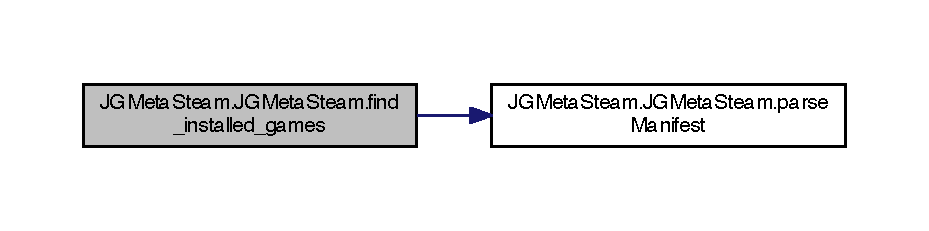
\includegraphics[width=350pt]{class_j_g_meta_steam_1_1_j_g_meta_steam_a8d61d2e7e511e8001ad0de115266ce5b_cgraph}
\end{center}
\end{figure}


\hypertarget{class_j_g_meta_steam_1_1_j_g_meta_steam_ad61c5083ca71695f1d5945707c0857ae}{\index{J\+G\+Meta\+Steam\+::\+J\+G\+Meta\+Steam@{J\+G\+Meta\+Steam\+::\+J\+G\+Meta\+Steam}!find\+\_\+steam@{find\+\_\+steam}}
\index{find\+\_\+steam@{find\+\_\+steam}!J\+G\+Meta\+Steam\+::\+J\+G\+Meta\+Steam@{J\+G\+Meta\+Steam\+::\+J\+G\+Meta\+Steam}}
\subsubsection[{find\+\_\+steam}]{\setlength{\rightskip}{0pt plus 5cm}def J\+G\+Meta\+Steam.\+J\+G\+Meta\+Steam.\+find\+\_\+steam (
\begin{DoxyParamCaption}
\item[{}]{self}
\end{DoxyParamCaption}
)}}\label{class_j_g_meta_steam_1_1_j_g_meta_steam_ad61c5083ca71695f1d5945707c0857ae}


Find Steam. 

Searches the filesystem for where steam is

This allows command line calling of games \begin{DoxyRefDesc}{Todo}
\item[\hyperlink{todo__todo000002}{Todo}]implement \end{DoxyRefDesc}
\hypertarget{class_j_g_meta_steam_1_1_j_g_meta_steam_a589b698d11b79971bde98e61c3ab25c3}{\index{J\+G\+Meta\+Steam\+::\+J\+G\+Meta\+Steam@{J\+G\+Meta\+Steam\+::\+J\+G\+Meta\+Steam}!find\+\_\+steam\+\_\+folders@{find\+\_\+steam\+\_\+folders}}
\index{find\+\_\+steam\+\_\+folders@{find\+\_\+steam\+\_\+folders}!J\+G\+Meta\+Steam\+::\+J\+G\+Meta\+Steam@{J\+G\+Meta\+Steam\+::\+J\+G\+Meta\+Steam}}
\subsubsection[{find\+\_\+steam\+\_\+folders}]{\setlength{\rightskip}{0pt plus 5cm}def J\+G\+Meta\+Steam.\+J\+G\+Meta\+Steam.\+find\+\_\+steam\+\_\+folders (
\begin{DoxyParamCaption}
\item[{}]{self}
\end{DoxyParamCaption}
)}}\label{class_j_g_meta_steam_1_1_j_g_meta_steam_a589b698d11b79971bde98e61c3ab25c3}


Find Steam folders. 

Searches the filesystem for where steam games are

This enables searching for installed games \begin{DoxyRefDesc}{Todo}
\item[\hyperlink{todo__todo000003}{Todo}]implement \end{DoxyRefDesc}
\hypertarget{class_j_g_meta_steam_1_1_j_g_meta_steam_abcb0c088945b4058f711e62e91679664}{\index{J\+G\+Meta\+Steam\+::\+J\+G\+Meta\+Steam@{J\+G\+Meta\+Steam\+::\+J\+G\+Meta\+Steam}!game\+\_\+info@{game\+\_\+info}}
\index{game\+\_\+info@{game\+\_\+info}!J\+G\+Meta\+Steam\+::\+J\+G\+Meta\+Steam@{J\+G\+Meta\+Steam\+::\+J\+G\+Meta\+Steam}}
\subsubsection[{game\+\_\+info}]{\setlength{\rightskip}{0pt plus 5cm}def J\+G\+Meta\+Steam.\+J\+G\+Meta\+Steam.\+game\+\_\+info (
\begin{DoxyParamCaption}
\item[{}]{self, }
\item[{}]{gameid}
\end{DoxyParamCaption}
)}}\label{class_j_g_meta_steam_1_1_j_g_meta_steam_abcb0c088945b4058f711e62e91679664}


Outputs information on a game. 

Takes a gameid, searches the found games, returns all information


\begin{DoxyParams}{Parameters}
{\em gameid} & The numeric representation of a game \\
\hline
\end{DoxyParams}
\begin{DoxyRefDesc}{Todo}
\item[\hyperlink{todo__todo000005}{Todo}]implement \end{DoxyRefDesc}
\hypertarget{class_j_g_meta_steam_1_1_j_g_meta_steam_a65974fc7a029c0b970f5915f2c9de0fd}{\index{J\+G\+Meta\+Steam\+::\+J\+G\+Meta\+Steam@{J\+G\+Meta\+Steam\+::\+J\+G\+Meta\+Steam}!import\+Json@{import\+Json}}
\index{import\+Json@{import\+Json}!J\+G\+Meta\+Steam\+::\+J\+G\+Meta\+Steam@{J\+G\+Meta\+Steam\+::\+J\+G\+Meta\+Steam}}
\subsubsection[{import\+Json}]{\setlength{\rightskip}{0pt plus 5cm}def J\+G\+Meta\+Steam.\+J\+G\+Meta\+Steam.\+import\+Json (
\begin{DoxyParamCaption}
\item[{}]{self}
\end{DoxyParamCaption}
)}}\label{class_j_g_meta_steam_1_1_j_g_meta_steam_a65974fc7a029c0b970f5915f2c9de0fd}


import saved and parsed data 

\hypertarget{class_j_g_meta_steam_1_1_j_g_meta_steam_a585febb64a52bd71d389c40eae1c6560}{\index{J\+G\+Meta\+Steam\+::\+J\+G\+Meta\+Steam@{J\+G\+Meta\+Steam\+::\+J\+G\+Meta\+Steam}!open\+Visualisation@{open\+Visualisation}}
\index{open\+Visualisation@{open\+Visualisation}!J\+G\+Meta\+Steam\+::\+J\+G\+Meta\+Steam@{J\+G\+Meta\+Steam\+::\+J\+G\+Meta\+Steam}}
\subsubsection[{open\+Visualisation}]{\setlength{\rightskip}{0pt plus 5cm}def J\+G\+Meta\+Steam.\+J\+G\+Meta\+Steam.\+open\+Visualisation (
\begin{DoxyParamCaption}
\item[{}]{self}
\end{DoxyParamCaption}
)}}\label{class_j_g_meta_steam_1_1_j_g_meta_steam_a585febb64a52bd71d389c40eae1c6560}


system call to visualisation d3 html page 

\hypertarget{class_j_g_meta_steam_1_1_j_g_meta_steam_ae6af3be62be13a876f6cae553961381d}{\index{J\+G\+Meta\+Steam\+::\+J\+G\+Meta\+Steam@{J\+G\+Meta\+Steam\+::\+J\+G\+Meta\+Steam}!parse\+Manifest@{parse\+Manifest}}
\index{parse\+Manifest@{parse\+Manifest}!J\+G\+Meta\+Steam\+::\+J\+G\+Meta\+Steam@{J\+G\+Meta\+Steam\+::\+J\+G\+Meta\+Steam}}
\subsubsection[{parse\+Manifest}]{\setlength{\rightskip}{0pt plus 5cm}def J\+G\+Meta\+Steam.\+J\+G\+Meta\+Steam.\+parse\+Manifest (
\begin{DoxyParamCaption}
\item[{}]{self, }
\item[{}]{manifest}
\end{DoxyParamCaption}
)}}\label{class_j_g_meta_steam_1_1_j_g_meta_steam_ae6af3be62be13a876f6cae553961381d}


Open and parse a manifest to extract starting information. 

\hypertarget{class_j_g_meta_steam_1_1_j_g_meta_steam_af5e7d7eec9571c54e744f66ee76ea9b4}{\index{J\+G\+Meta\+Steam\+::\+J\+G\+Meta\+Steam@{J\+G\+Meta\+Steam\+::\+J\+G\+Meta\+Steam}!parse\+Store@{parse\+Store}}
\index{parse\+Store@{parse\+Store}!J\+G\+Meta\+Steam\+::\+J\+G\+Meta\+Steam@{J\+G\+Meta\+Steam\+::\+J\+G\+Meta\+Steam}}
\subsubsection[{parse\+Store}]{\setlength{\rightskip}{0pt plus 5cm}def J\+G\+Meta\+Steam.\+J\+G\+Meta\+Steam.\+parse\+Store (
\begin{DoxyParamCaption}
\item[{}]{self, }
\item[{}]{soup, }
\item[{}]{gameid}
\end{DoxyParamCaption}
)}}\label{class_j_g_meta_steam_1_1_j_g_meta_steam_af5e7d7eec9571c54e744f66ee76ea9b4}


Parses html assuming its a steam store page. 



Here is the call graph for this function\+:\nopagebreak
\begin{figure}[H]
\begin{center}
\leavevmode
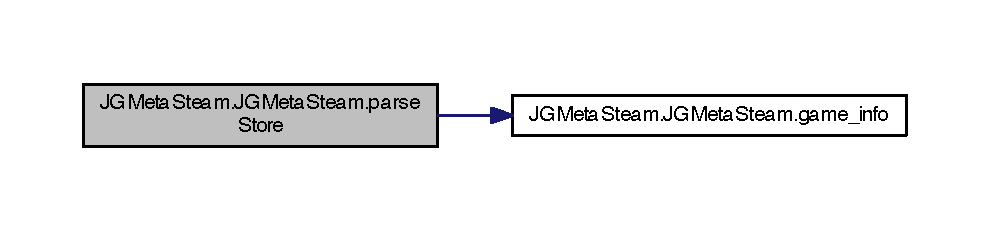
\includegraphics[width=350pt]{class_j_g_meta_steam_1_1_j_g_meta_steam_af5e7d7eec9571c54e744f66ee76ea9b4_cgraph}
\end{center}
\end{figure}


\hypertarget{class_j_g_meta_steam_1_1_j_g_meta_steam_ada308bf6bdb3bd2acedaa704cf34139f}{\index{J\+G\+Meta\+Steam\+::\+J\+G\+Meta\+Steam@{J\+G\+Meta\+Steam\+::\+J\+G\+Meta\+Steam}!random\+Game@{random\+Game}}
\index{random\+Game@{random\+Game}!J\+G\+Meta\+Steam\+::\+J\+G\+Meta\+Steam@{J\+G\+Meta\+Steam\+::\+J\+G\+Meta\+Steam}}
\subsubsection[{random\+Game}]{\setlength{\rightskip}{0pt plus 5cm}def J\+G\+Meta\+Steam.\+J\+G\+Meta\+Steam.\+random\+Game (
\begin{DoxyParamCaption}
\item[{}]{self}
\end{DoxyParamCaption}
)}}\label{class_j_g_meta_steam_1_1_j_g_meta_steam_ada308bf6bdb3bd2acedaa704cf34139f}


Here is the call graph for this function\+:
\nopagebreak
\begin{figure}[H]
\begin{center}
\leavevmode
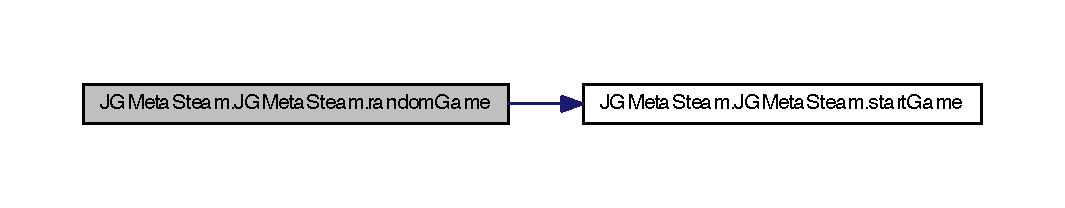
\includegraphics[width=350pt]{class_j_g_meta_steam_1_1_j_g_meta_steam_ada308bf6bdb3bd2acedaa704cf34139f_cgraph}
\end{center}
\end{figure}


\hypertarget{class_j_g_meta_steam_1_1_j_g_meta_steam_a6a34f50ae4397170316bee6f81cabbe9}{\index{J\+G\+Meta\+Steam\+::\+J\+G\+Meta\+Steam@{J\+G\+Meta\+Steam\+::\+J\+G\+Meta\+Steam}!scrape\+\_\+info@{scrape\+\_\+info}}
\index{scrape\+\_\+info@{scrape\+\_\+info}!J\+G\+Meta\+Steam\+::\+J\+G\+Meta\+Steam@{J\+G\+Meta\+Steam\+::\+J\+G\+Meta\+Steam}}
\subsubsection[{scrape\+\_\+info}]{\setlength{\rightskip}{0pt plus 5cm}def J\+G\+Meta\+Steam.\+J\+G\+Meta\+Steam.\+scrape\+\_\+info (
\begin{DoxyParamCaption}
\item[{}]{self, }
\item[{}]{gameid}
\end{DoxyParamCaption}
)}}\label{class_j_g_meta_steam_1_1_j_g_meta_steam_a6a34f50ae4397170316bee6f81cabbe9}


Scrapes the steam store for a games information. 

Takes a gameid, looks up its steam page, filters and adds to the games datastructure


\begin{DoxyParams}{Parameters}
{\em gameid} & The numeric representation of a game \\
\hline
\end{DoxyParams}
\begin{DoxyRefDesc}{Todo}
\item[\hyperlink{todo__todo000007}{Todo}]implement \end{DoxyRefDesc}


Here is the call graph for this function\+:\nopagebreak
\begin{figure}[H]
\begin{center}
\leavevmode
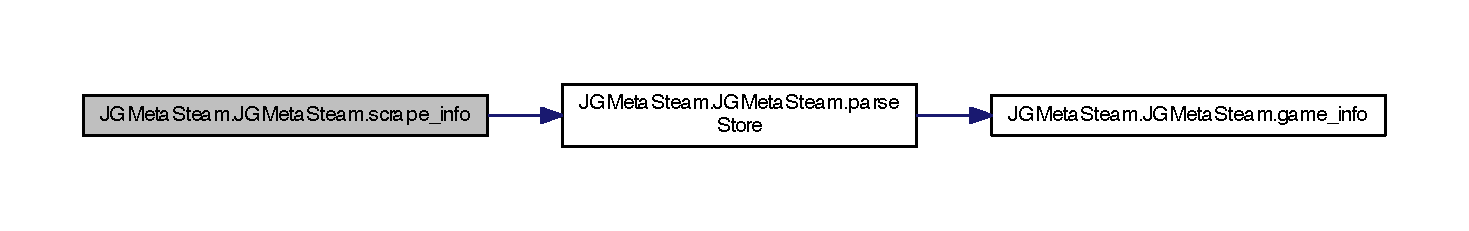
\includegraphics[width=350pt]{class_j_g_meta_steam_1_1_j_g_meta_steam_a6a34f50ae4397170316bee6f81cabbe9_cgraph}
\end{center}
\end{figure}


\hypertarget{class_j_g_meta_steam_1_1_j_g_meta_steam_a7138734ce6e670d875b7c0d7367c2e7e}{\index{J\+G\+Meta\+Steam\+::\+J\+G\+Meta\+Steam@{J\+G\+Meta\+Steam\+::\+J\+G\+Meta\+Steam}!start\+Game@{start\+Game}}
\index{start\+Game@{start\+Game}!J\+G\+Meta\+Steam\+::\+J\+G\+Meta\+Steam@{J\+G\+Meta\+Steam\+::\+J\+G\+Meta\+Steam}}
\subsubsection[{start\+Game}]{\setlength{\rightskip}{0pt plus 5cm}def J\+G\+Meta\+Steam.\+J\+G\+Meta\+Steam.\+start\+Game (
\begin{DoxyParamCaption}
\item[{}]{self, }
\item[{}]{gameid}
\end{DoxyParamCaption}
)}}\label{class_j_g_meta_steam_1_1_j_g_meta_steam_a7138734ce6e670d875b7c0d7367c2e7e}


start a user defined game, based on gameid or choose a random one if none defined 



\subsection{Member Data Documentation}
\hypertarget{class_j_g_meta_steam_1_1_j_g_meta_steam_ad9770696b4a76d5706f5bf5f87a54f4b}{\index{J\+G\+Meta\+Steam\+::\+J\+G\+Meta\+Steam@{J\+G\+Meta\+Steam\+::\+J\+G\+Meta\+Steam}!steam\+Location@{steam\+Location}}
\index{steam\+Location@{steam\+Location}!J\+G\+Meta\+Steam\+::\+J\+G\+Meta\+Steam@{J\+G\+Meta\+Steam\+::\+J\+G\+Meta\+Steam}}
\subsubsection[{steam\+Location}]{\setlength{\rightskip}{0pt plus 5cm}J\+G\+Meta\+Steam.\+J\+G\+Meta\+Steam.\+steam\+Location}}\label{class_j_g_meta_steam_1_1_j_g_meta_steam_ad9770696b4a76d5706f5bf5f87a54f4b}


The documentation for this class was generated from the following file\+:\begin{DoxyCompactItemize}
\item 
\hyperlink{_j_g_meta_steam_8py}{J\+G\+Meta\+Steam.\+py}\end{DoxyCompactItemize}

\hypertarget{class_j_g_meta_steam}{\section{J\+G\+Meta\+Steam Class Reference}
\label{class_j_g_meta_steam}\index{J\+G\+Meta\+Steam@{J\+G\+Meta\+Steam}}
}


\subsection{Detailed Description}
\begin{DoxyRefDesc}{Todo}
\item[\hyperlink{todo__todo000001}{Todo}]sort the globbing 

sort the web calling and parsing 

sort json import and e3xport 

sort the random game execution \end{DoxyRefDesc}


The documentation for this class was generated from the following file\+:\begin{DoxyCompactItemize}
\item 
\hyperlink{_j_g_meta_steam_8py}{J\+G\+Meta\+Steam.\+py}\end{DoxyCompactItemize}

\chapter{File Documentation}
\hypertarget{all_game_parse_8py}{\section{all\+Game\+Parse.\+py File Reference}
\label{all_game_parse_8py}\index{all\+Game\+Parse.\+py@{all\+Game\+Parse.\+py}}
}
\subsection*{Namespaces}
\begin{DoxyCompactItemize}
\item 
 \hyperlink{namespaceall_game_parse}{all\+Game\+Parse}
\end{DoxyCompactItemize}
\subsection*{Variables}
\begin{DoxyCompactItemize}
\item 
tuple \hyperlink{namespaceall_game_parse_a0edb49935fe4f03afaeda24b26701cac}{all\+Game\+Parse.\+cj} = Cookie\+Jar()
\item 
tuple \hyperlink{namespaceall_game_parse_a1805ba57761718ea195891b56adac271}{all\+Game\+Parse.\+gameid} = str(91310)
\item 
string \hyperlink{namespaceall_game_parse_af48967d69b2b722ff05ad284da8f4bfe}{all\+Game\+Parse.\+url} = \char`\"{}http\+://steamcommunity.\+com/id/belial4296/games/\char`\"{}
\item 
tuple \hyperlink{namespaceall_game_parse_a1cefe9996713674c46f624baa334280d}{all\+Game\+Parse.\+opener} = urllib2.\+build\+\_\+opener(urllib2.\+H\+T\+T\+P\+Cookie\+Processor(cj))
\item 
dictionary \hyperlink{namespaceall_game_parse_a25e198ad333ea40e9d4eca9e8ac0ce59}{all\+Game\+Parse.\+values}
\item 
tuple \hyperlink{namespaceall_game_parse_a8b0c2752622015229ec7c131f733b221}{all\+Game\+Parse.\+data} = urllib.\+urlencode(values)
\item 
tuple \hyperlink{namespaceall_game_parse_a5bfed9efebbc641889b00e0505c4a4ae}{all\+Game\+Parse.\+req} = urllib2.\+Request(url,data)
\item 
tuple \hyperlink{namespaceall_game_parse_a7bbf07843967c52d1d807c64b6d009d0}{all\+Game\+Parse.\+response} = opener.\+open(req)
\item 
tuple \hyperlink{namespaceall_game_parse_a8dd688b6fdf0d5dc75fd1052e88199da}{all\+Game\+Parse.\+html} = response.\+read()
\item 
tuple \hyperlink{namespaceall_game_parse_a6b3a0dce9a39a129a40c94cf1bd1ee9b}{all\+Game\+Parse.\+soup} = Beautiful\+Soup(html)
\item 
tuple \hyperlink{namespaceall_game_parse_a43d3a3e6df161dd6b906b25ba68e3f08}{all\+Game\+Parse.\+rows} = soup.\+find(id=\char`\"{}games\+\_\+list\+\_\+rows\char`\"{})
\item 
tuple \hyperlink{namespaceall_game_parse_a2bdbbc305ed8beb518d32abaf8866039}{all\+Game\+Parse.\+row} = rows.\+find(id=\char`\"{}game\+\_\+56400\char`\"{})
\end{DoxyCompactItemize}

\hypertarget{_j_g_meta_steam_8py}{\section{J\+G\+Meta\+Steam.\+py File Reference}
\label{_j_g_meta_steam_8py}\index{J\+G\+Meta\+Steam.\+py@{J\+G\+Meta\+Steam.\+py}}
}


The \hyperlink{namespacemeta_steam}{meta\+Steam} class that does the heavy lifting.  


\subsection*{Classes}
\begin{DoxyCompactItemize}
\item 
class \hyperlink{class_j_g_meta_steam_1_1_j_g_meta_steam}{J\+G\+Meta\+Steam.\+J\+G\+Meta\+Steam}
\end{DoxyCompactItemize}
\subsection*{Namespaces}
\begin{DoxyCompactItemize}
\item 
 \hyperlink{namespace_j_g_meta_steam}{J\+G\+Meta\+Steam}
\end{DoxyCompactItemize}


\subsection{Detailed Description}
The \hyperlink{namespacemeta_steam}{meta\+Steam} class that does the heavy lifting. 


\hypertarget{meta_steam_8py}{\section{meta\+Steam.\+py File Reference}
\label{meta_steam_8py}\index{meta\+Steam.\+py@{meta\+Steam.\+py}}
}


Python reimplementation of perl metasteam.  


\subsection*{Namespaces}
\begin{DoxyCompactItemize}
\item 
 \hyperlink{namespacemeta_steam}{meta\+Steam}
\end{DoxyCompactItemize}
\subsection*{Functions}
\begin{DoxyCompactItemize}
\item 
def \hyperlink{namespacemeta_steam_ac19e5b2b462300c1ab5a320900d7c93b}{meta\+Steam.\+printall\+Games}
\begin{DoxyCompactList}\small\item\em user input -\/$>$ function \end{DoxyCompactList}\item 
def \hyperlink{namespacemeta_steam_a2d6ff00a0d1702a02ffaea0fddf84cb7}{meta\+Steam.\+print\+Info\+For\+Game}
\begin{DoxyCompactList}\small\item\em prints all the info on a single game \end{DoxyCompactList}\item 
def \hyperlink{namespacemeta_steam_abcf03e99fea34697691c1e3b5572aa27}{meta\+Steam.\+scrape\+All\+Games}
\begin{DoxyCompactList}\small\item\em get all games, and scrape them slowly \end{DoxyCompactList}\item 
def \hyperlink{namespacemeta_steam_a926c83f223c5f1d110246bc448fcc1e3}{meta\+Steam.\+scrape\+And\+Print\+Game}
\item 
def \hyperlink{namespacemeta_steam_a4fd0814c8d2980d8cdc7baed0e733588}{meta\+Steam.\+start\+Game}
\begin{DoxyCompactList}\small\item\em start a specific or random game (for later\+: playlists) \end{DoxyCompactList}\item 
def \hyperlink{namespacemeta_steam_aba7bea32668601ae15aebcd436128c90}{meta\+Steam.\+print\+Help}
\begin{DoxyCompactList}\small\item\em print the help documentation \end{DoxyCompactList}\item 
def \hyperlink{namespacemeta_steam_a012c898f91eb4ce14f9e16b1bbe76c69}{meta\+Steam.\+export\+Json}
\begin{DoxyCompactList}\small\item\em export game information to json \end{DoxyCompactList}\item 
def \hyperlink{namespacemeta_steam_ae2c97e161b9e6d6b65daad8b83fe4d3c}{meta\+Steam.\+import\+Json}
\item 
def \hyperlink{namespacemeta_steam_af9130303bff378cfcf624a0302102398}{meta\+Steam.\+main}
\begin{DoxyCompactList}\small\item\em The user interaction loop. \end{DoxyCompactList}\end{DoxyCompactItemize}
\subsection*{Variables}
\begin{DoxyCompactItemize}
\item 
dictionary \hyperlink{namespacemeta_steam_a05799bd182d0bf8b0e97b1e36b1e4ed4}{meta\+Steam.\+commands}
\end{DoxyCompactItemize}


\subsection{Detailed Description}
Python reimplementation of perl metasteam. 

\begin{DoxyAuthor}{Author}
John Grey \href{mailto:jgrey@ucsc.soe.edu}{\tt jgrey@ucsc.\+soe.\+edu} 
\end{DoxyAuthor}
\begin{DoxyVersion}{Version}
0.\+1 
\end{DoxyVersion}
\begin{DoxyDate}{Date}

\end{DoxyDate}

\hypertarget{test_request_8py}{\section{test\+Request.\+py File Reference}
\label{test_request_8py}\index{test\+Request.\+py@{test\+Request.\+py}}
}
\subsection*{Namespaces}
\begin{DoxyCompactItemize}
\item 
 \hyperlink{namespacetest_request}{test\+Request}
\end{DoxyCompactItemize}
\subsection*{Variables}
\begin{DoxyCompactItemize}
\item 
tuple \hyperlink{namespacetest_request_afd477347e61eaf087de75394b8249088}{test\+Request.\+cj} = Cookie\+Jar()
\item 
tuple \hyperlink{namespacetest_request_ad59cb201aaea659d05de3a976c43d2d0}{test\+Request.\+gameid} = str(91310)
\item 
string \hyperlink{namespacetest_request_a503c8624234f46b468f9d0b807d63cb0}{test\+Request.\+url} = \char`\"{}http\+://store.\+steampowered.\+com/app/\char`\"{}
\item 
tuple \hyperlink{namespacetest_request_a32d478514621667126784650159375ae}{test\+Request.\+opener} = urllib2.\+build\+\_\+opener(urllib2.\+H\+T\+T\+P\+Cookie\+Processor(cj))
\item 
tuple \hyperlink{namespacetest_request_a82a62563089eee6f274889ef4cda4c83}{test\+Request.\+response} = urllib2.\+urlopen(url)
\item 
tuple \hyperlink{namespacetest_request_a8f35331152c0a50dcf80c4e88192e928}{test\+Request.\+html} = response.\+read()
\item 
tuple \hyperlink{namespacetest_request_abdcf7c50bc605e36463827591ea27597}{test\+Request.\+soup} = Beautiful\+Soup(html)
\item 
tuple \hyperlink{namespacetest_request_a577a66202d87bdc38bab9969bd0b0be8}{test\+Request.\+agecheckform} = soup.\+find\+\_\+all(id=\char`\"{}agecheck\+\_\+form\char`\"{})
\item 
tuple \hyperlink{namespacetest_request_a9dd80d2ee25233da56bf90ee2b6562f8}{test\+Request.\+forminput} = soup.\+find\+\_\+all('input',type=\char`\"{}hidden\char`\"{})
\item 
list \hyperlink{namespacetest_request_ac0dc477bbe063b2dc0a1e8fab9086a45}{test\+Request.\+fin\+Val} = forminput\mbox{[}1\mbox{]}
\item 
dictionary \hyperlink{namespacetest_request_ad045126755bc1baa0a4cacb58d77b4a1}{test\+Request.\+values}
\item 
tuple \hyperlink{namespacetest_request_aa2da30dcafd8fe42c8408aba77c7e70f}{test\+Request.\+data} = urllib.\+urlencode(values)
\item 
tuple \hyperlink{namespacetest_request_a5db18cf7ac0523c1940da68f3301fc49}{test\+Request.\+req} = urllib2.\+Request(url,data)
\item 
tuple \hyperlink{namespacetest_request_a52e13bffa1978df832b6676e9e492fe0}{test\+Request.\+all\+Tags} = soup.\+find\+\_\+all(class\+\_\+=\char`\"{}app\+\_\+tag\char`\"{})
\end{DoxyCompactItemize}

%--- End generated contents ---

% Index
\newpage
\phantomsection
\addcontentsline{toc}{chapter}{Index}
\printindex

\end{document}
